\chapter{Alternativas arquitecturas}
\label{anexo-a}

En el proceso de diseño de la arquitectura software del proyecto se evaluan distintas opciones con el objetivo de seleccionar la más adecuada para cumplir con los objetivos y requisitos de la empresa. Los principales motivos de este análisis son:

\begin{itemize}
    \item Tener o no un middleware que actúe de servidor web para comunicar la aplicación web y la aplicación existente de Ibernex (Helpnex).
    \item El problema de compatibilidad de utilizar SignalR (Véase  \hyperref[anexo-b]{Anexo B}) para comunicar la aplicación de Ibernex y la aplicación web.
\end{itemize}

En un principio, el diseño de arquitetura propuesto por la empresa es el que se puede ver en la \textit{Figura A.1}. Lo que proponían incluía un middleware para realizar una autenticación mediante API REST utilizando JWT (Véase \hyperref[anexo-c]{Anexo C}) y la comunicación entre los componentes de la arquitecura con websockets utilizando SignalR.  

\begin{figure}[!h]
    \centering
    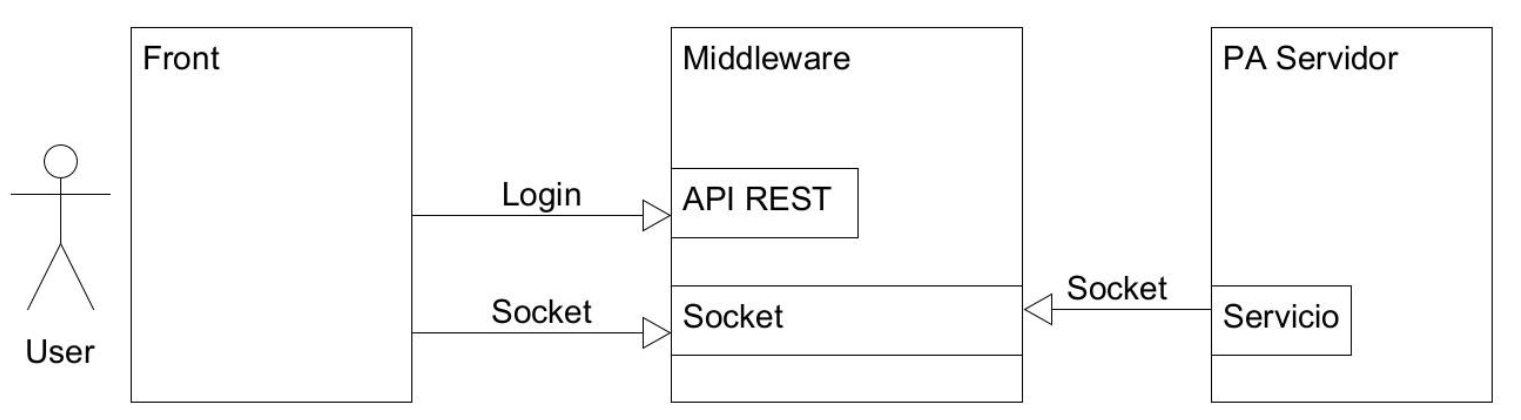
\includegraphics[width=15cm]{Imagenes/Descripcion-arquitectura}
    \caption{Diagrama propuesto por la empresa}
    \label{fig:descripcion-arquitectura}
\end{figure}

Durante el desarrollo del proyecto la empresa decide que no es necesario utilizar una autenticación por JWT en estos momentos, por lo que tener un middleware con API REST no tiene sentido si el resto de la comunicación se puede hacer por websockets.\\

Ahora, lo que se necesita es la comunicación mediante websockets entre el nuevo servicio implementado en PAServidor y la aplicación web. La empresa había propuesto utilizar SignalR como tecnología para realizar dicha comunicación. El problema se encuentra cuando haciendo pruebas de funcionamiento, para utilizarla en la implementación, se ve la incompatibilidad de SignalR con .NET Framework 4.8 que es la tecnología con la que se implementa Helpnex.\\

Por esta razón, se buscan alternativas para utilizar SignalR. Las propuesta que se le proponen a la empresa son: 
\begin{enumerate}
    \item Seguir utilizando un Middleware (sin API REST) que siga utilizando SignalR para comunicarse con el frontend React y websockets (sin SignalR) para comunicarse con PAServidor.
    \item Realizar la comunicación entre aplicación web y servicio de PAServidor directamente con websockets sin utilizar SignalR.
\end{enumerate}

Para la primera opción el diagrama de despliegue que se propone a la empresa es el que se puede ver en la \textit{Figura A.2}. Aquí se pueden ver una aplicación web React, un servidor web que hace de proxy con ASP .NET Core (que sí es compatible con SignalR) y PAServidor, como tres proyectos independientes. Pero, para esta solución, la empresa pensaba que lo que se haría sería algo similar teniendo un único proyecto incluyendo la aplicación web y el servidor web (un proyecto en el entorno de desarrollo de Microsoft Visual Studio en el que se crea una aplicación ASP.NET Core con React \cite{vs-project} ) y por otro lado el PAServidor (Véase \textit{Figura A.3})\\

\begin{figure}[H]
    \centering
    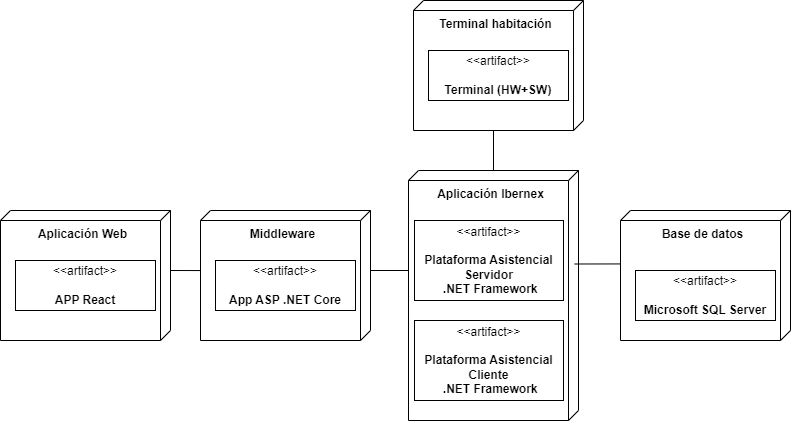
\includegraphics[width=15cm]{Imagenes/Arquitectura-despliegue-2}
    \caption{Diagrama de despliegue con Middleware}
    \label{fig:despliegue-2}
\end{figure}


\begin{figure}[H]
    \centering
    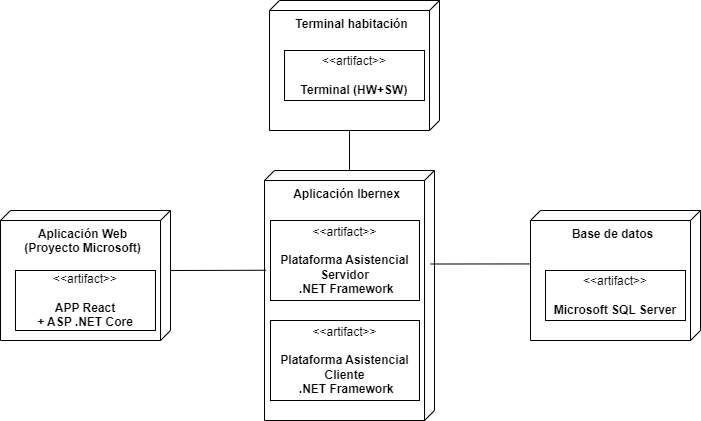
\includegraphics[width=15cm]{Imagenes/Arquitectura-despliegue-3}
    \caption{Diagrama de despliegue - único proyecto}
    \label{fig:despliegue-3}
\end{figure}

Finalmente, se decide junto con la empresa que es innecesario tener un servidor web si la comunicación se puede hacer directamente entre la aplicación web y PAServidor, aunque sea sin utilizar SignalR (ya que la empresa no contaba con la incompatibilidad).\\

Por esta razón, para la segunda opción el diagrama de despliegue que se propone a la empresa es el de la arquitectura final elegida para el proyecto que es la que se puede ver en la \hyperref[fig:despliegue]{\textit{Figura 2.1}} que se encuentra en una de las secciones anteriores.








